\section{问题三建模与求解}

\subsection{数据预处理}

通过Pandas库进行数据读取,使用isnull函数查找数据中的缺失值,对于附件表单3中缺失值进行补0,并对于表中样本化学成分含量求和,均满足85\%—105\%,无需对数据进行删减。

\subsection{未知类别文物预测模型}

\subsubsection{模型准备}

模型选择前文从附件表二处理后(补齐缺失值,删除不满足条件只值)的数据中提取的14个化学成分和风化情况这15个特征。以原数据为标准,将数据进行标准化将数据处理到0到1之间。对风化情况进行独热编码。

\subsubsection{模型建立}

投票(voting)在集成学习的分类算法中被广泛运用,投票主要运用软投票(soft voting)是一种对于各基分类器效果融合的模型。本文所选择的4个基分类器分别为线性判别分析、决策树、朴素贝叶斯以及支持向量机。并用voting进行基分类器融合得到一个强分类器。

\begin{figure}[H] 
	\centering %图片居中
	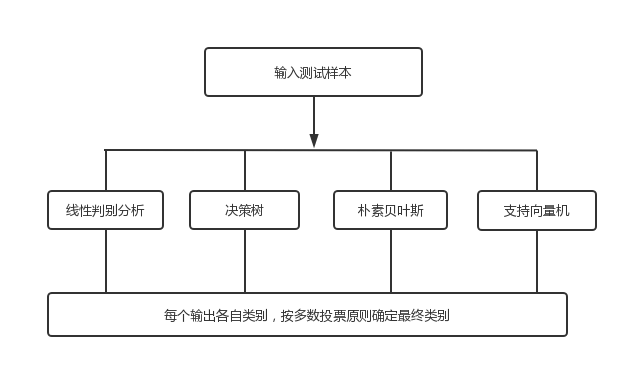
\includegraphics[width=0.7\textwidth]{19.png} %插入图片,[]中设置图片大小,{}中是图片文件名
	\caption{Voting原理} %最终文档中希望显示的图片标题
	\label{Fig.main20} %用于文内引用的标签
\end{figure}



\subsubsection{模型求解}

建立线性判别分析、决策树、朴素贝叶斯以及支持向量机四个性能优良的传统机器学习分类模型,并将训练集分别投入四个模型进行模型训练,通过比较交叉验证后的得分结果,发现四个模型性能均远超过随机分类(成功率0.5)。


\begin{table}[H]
	\centering
	\begin{tabular}{c c} 
		\toprule[1.5pt]
		分类器 & 综合准确率 \\
		\midrule[1pt]
		线性判别分析 & 0.971429 \\
		决策树 & 0.995382 \\
		朴素贝叶斯 & 0.985714 \\
		支持向量机 & 0.985714 \\
		\toprule[1.5pt]
	\end{tabular}
\caption{基分类器评分}
\end{table}

从上表可以看出四种基分类器效果都不错,对于测试集的数据训练准确率都在百分之九十七以上,都是比较好的分类预测模型。

然而四个分类器的分类效果各不相同,所以本着训练性能最优良分类器的原则,本文使用基于结果进行模型融合的VotingClassifier投票算法对四个模型进行融合,公式为:


\begin{equation}
    {{W}_{i}}=\frac{accurac{{y}_{i}}}{\sum\limits_{i=1}^{5}{accurac{{y}_{i}}}}
\end{equation}

软投票的分类结果如下表:

\begin{table}[H]
	\centering
	\begin{tabular}{c c} 
		\toprule[1.5pt]
		分类器 & 综合准确率 \\
		\midrule[1pt]
		VotingClassifier & 1 \\
		\toprule[1.5pt]
	\end{tabular}
\caption{分类结果表}
\end{table}

最后得到了分类预测成功率为1的“完美模型”。
下面对于该分类模型进行评价,利用混淆矩阵热力图如下:


\begin{figure}[H] 
	\centering %图片居中
	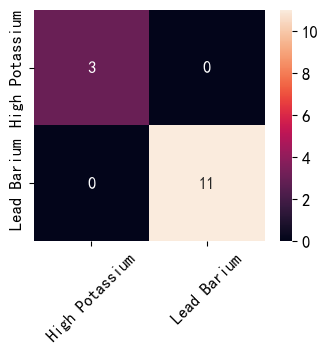
\includegraphics[width=0.7\textwidth]{20.png} %插入图片,[]中设置图片大小,{}中是图片文件名
	\caption{VotingClassifier混淆矩阵热力图} %最终文档中希望显示的图片标题
	\label{Fig.main21} %用于文内引用的标签
\end{figure}


可以看出VotingClassifier分类模型非常完美,是一个非常好的分类器。再基于混淆矩阵的方法对该分类模型进行评价,结合对测试集的预测结果和测试集自身标签、通过计算得到模型的精确度得到如下指标:

\begin{table}[H]
	\centering
	\begin{tabular}{c c c c c} 
		\toprule[1.5pt]
		 & 精确度 & 召回率 & F1分数 & 支持率 \\
        \midrule[1pt]
		铅钡 & 1 & 1 & 1 & 1 \\
		\hline
		高钾 & 1 & 1 & 1 & 1 \\
		\hline
		加权平均 & 1 & 1 & 1 & 1 \\
		\toprule[1.5pt]
	\end{tabular}
\caption{评分数据表}
\end{table}

通过表11可以看到该分类器确实非常“完美”。
利用该模型对预处理过后的附件表三进行分类预测,预测结果如下:



\begin{table}[H]
	\centering
	\begin{tabular}{c c} 
		\toprule[1.5pt]
		高钾玻璃 & $A_1,A_6,A_7$ \\
		\midrule[1pt]
		铅钡玻璃 & $A_2,A_3,A_4,A_5,A_8$ \\
		\toprule[1.5pt]
	\end{tabular}
\caption{预测结果表}
\end{table}

由上表可以知道成功预测$A_1,A_6,A_7$为高钾玻璃,$A_2,A_3,A_4,A_5,A_8$为铅钡玻璃。


\subsection{模型敏感性分析}

利用公式(1)(2)得到每种化学成分的扰动值,带到模型中进行扰动检验,可以得到敏感阈值。对数据进行扰动,将扰动值重新带到模型中进行分类预测,得到干扰前后的结果图如下:


\begin{figure}[H] 
	\centering %图片居中
	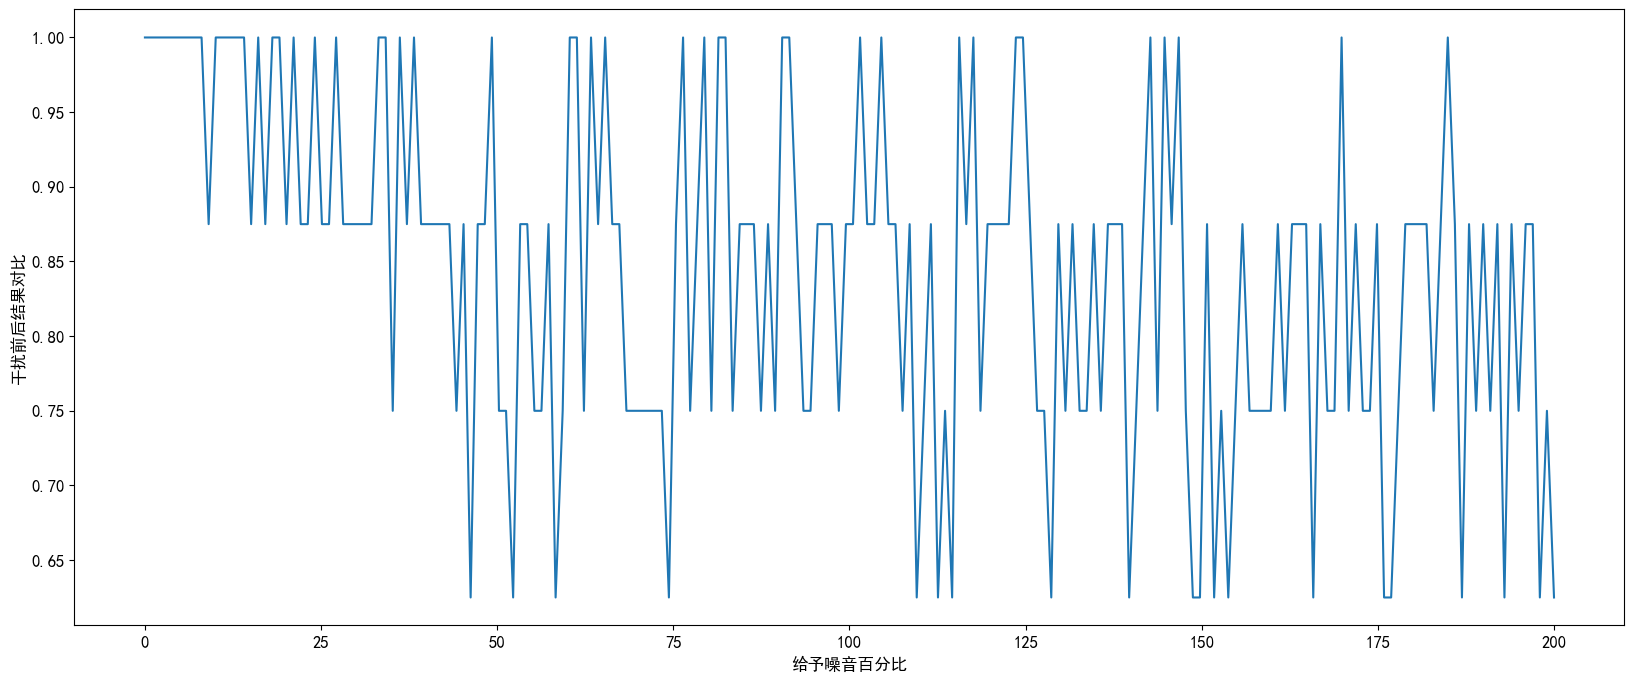
\includegraphics[width=0.7\textwidth]{21.png} %插入图片,[]中设置图片大小,{}中是图片文件名
	\caption{敏感性阈值图} %最终文档中希望显示的图片标题
	\label{Fig.main22} %用于文内引用的标签
\end{figure}

通过图21发现该模型的敏感性阈值d在(0,0.3)之间,模型的准确率都在85\%以上,当d在(0.3,0.45)之间模型的准确率都在75\%以上,而当d大于0.45时模型的准确率波动性大,预测准确率变化大,因此最好将数据的敏感性阈值控制在0.45以下。